\chapter{Определение географической принадлежности}

Рассматривая практические задачи, возникающие в контексте ДНК-идентификации, можно
выделить задачу определения географической принадлежности. Основным отличием данной задачи
от задачи определения этногеографической принадлежности является
большая гранулярность ожидаемых результатов, например, координаты населенного пункта проживания (места рождения)
неизвестного индивида. В данном случае множество координат-кандидатов не ограничено конечным множеством вариантов.

\section{Постановка задачи и метрики качества}
Задача определения географической принадлежности в общем виде может иметь следующий вид:
для заданного генотипа неизвестного индивида необходимо определить наиболее вероятные
места его происхождения. Очевидно, что данное определение носит весьма общий характер,
что в свою очередь заметно усложняет введение адекватных метрик качества.

Для создания более четкой формулировки, определение выше можно параметризовать, например,
с помощью следующих параметров:
\begin{itemize}
\item Погрешность (далее $d$) - некоторая величина, расстояние, характеризующая актуальность
предоставленных вариантов. Так, например, методы с погрешностью более 1000 км вряд ли
будут иметь спрос на территории Республики Беларусь. Мотивация для введения данного параметра проста:
чем точнее будут предоставленные варианты, тем лучше.

\item Максимальное количество кандидатов (далее $k$). Интуитивно понятно, что метод
определения географической принадлежности будет полезен на практике только при условии
предоставления ограниченного числа наиболее вероятных координат-кандидатов. Иначе можно было бы
просто покрыть равномерной решеткой всю целевую область -- истинные координаты были бы
в достаточной близости от одного из узлов.
\end{itemize}

Таким образом, можно немного сократить круг исследуемых задач:
нас интересуют методы, способные для некоторого генотипа $g$ предоставить список из $k$
наиболее вероятных координат-кандидатов согласно некоторой метрике качества $Q_{d}_{k} \left( C, c_{g} \right)$,
где $C = \left(c_{1}, ..., c_{k} \right)$ - множество координат-кандидатов, $c_{g}$ - истинные координаты.

На практике, вопрос подбора подходящих метрик для решения конкретных задач имеет большое значение.
Далее будут представлены некоторые варианты метрик качества:
\begin{itemize}
\item $Q^{hit}_{d}_{k} \left( C, c_{g} \right) = \max_{c \in C} \mathbbm{1} \left[ ||c - c_{g}|| <= d \right]$

Мотивация для применения данной метрики довольна проста: при фиксированном $d$
необходимо оценить вероятность того, что хотя бы один из кандидатов находится в достаточной близости от истинных координат генотипа.
Данная метрика дальше будет упоминаться как вероятность попадания (англ. hit probability).
При наличии некоторой тестовой выборки, нас будет интересовать максимизация данной метрики.

\item $Q^{precision}_{d}_{k} \left( C, c_{g} \right) = \frac{1}{k} \sum_{c \in C} \mathbbm{1} \left[ ||c - c_{g}|| <= d \right]$

Точность -- доля достаточно близких к истинным координатам генома координат-кандидатов. Данную метрику можно использовать в качестве дополнительной,
как некоторый аналог доверительного интервала для оценки качества представленных кандидатов, ведь более достоверными можно считать варианты в которых кандидаты сгруппированы
в виде нескольких блобов на карте, в отличие от равномерно распределенных по исследуемой территории кандидатов.

\item $Q^{mean}_{d}_{k} \left( C, c_{g} \right) = \frac{1}{k} \sum_{c \in C} ||c - c_{g}||$

Среднее расстояние от кандидатов до истинных координат.

\item $Q^{median}_{d}_{k} \left( C, c_{g} \right) = Median_{c \in C} ||c - c_{g}||$

Медиана расстояний от кандидатов до истинных координат.
\end{itemize}

Метрики выше подходят для оценки качества предсказания кандидатов для одного генотипа.
На практике возникает необходимость оценивать качество работы методов на множестве (например, тестовом)
генотипов. Довольно полезными оказываются следующие метрики:
\begin{itemize}
\item Покрытие -- мощность множества различных кандидатов, которые были предсказаны
для некоторого множества различных генотипов. Методы предсказания географической принадлежности должны обладать
достаточной вариабельностью. Если множества кандидатов для различных генотипов будут
обладать достаточно большим множеством общих кандидатов, то скорее всего роль генотипа
в генерации кандидатов играет недостаточно серьезную роль. При применении методов машинного обучения, либо
параметризованных методов, в таких ситуациях можно говорить о переобучении.
\item Компактность -- желательно, чтобы все кандидаты располагались в достаточной близости друг от друга.
Ясно, что данное требование может противоречить требованию наличия покрытия достаточной величины.
\end{itemize}

\section{Методы решения и тестирования}

Для разработки и тестирования методов решения задачи описанной в предыдущем разделе,
общая база генотипов была разделена на три части:

\begin{itemize}
\item Тренировочная выборка, далее $X_{train}$, содержит 1169 аннотированных генотипов
\item Валидационная выборка, далее $X_{val}$, содержит 62 аннотированных генотипа
\item Тестовая выборка, далее $X_{test}$, содержит 65 аннотированных генотипов
\end{itemize}

Каждый образец будем представлять в виде $(g_i, c^i_{g})$ - генотип и координаты населенного пункта,
где родился соответствующий индивид. Стоит отметить, что при разбиении общей базы генотипов
на выборки, скорее всего эффект на разбиение оказал влияние тот факт,
что из-за частоты встречаемости в исходной базе генотипов, с большей вероятностью
в валидационную и тестовую выборки могли попасть генотипы индивидов из густонаселенных районов.

Таким образом предполагаем, что валидационная выборка будет использоваться для подбора гиперпараметров,
либо отбора моделей. А финальное тестирование будет производиться на тестовой выборке.

Предлагается рассмотреть модели для определения географической принадлежности генотипов, удовлетворяющие следующим свойствам:
\begin{itemize}
\item Модель состоит из 2 компонент: генератора кандидатов и модуля для ранжирования кандидатов.
Декомпозиция такого рода позволит упростить проектирование и разработку каждой из компонент
\item Генератор кандидатов, используя тренировочную выборку $X_{train}$, создает множество потенциальных
координат-кандидатов
\item Множество кандидатов ранжируется, используя тренировочную выборку $X_{train}$ и генотип-запрос,
$k$ кандидатов с максимальным рангом используются в качестве предсказаний модели
\end{itemize}

Структурная схема представлена на рисунке $\left(\ref{image:geoloc_over}\right)$.

\begin{figure}[h]
\begin{center}
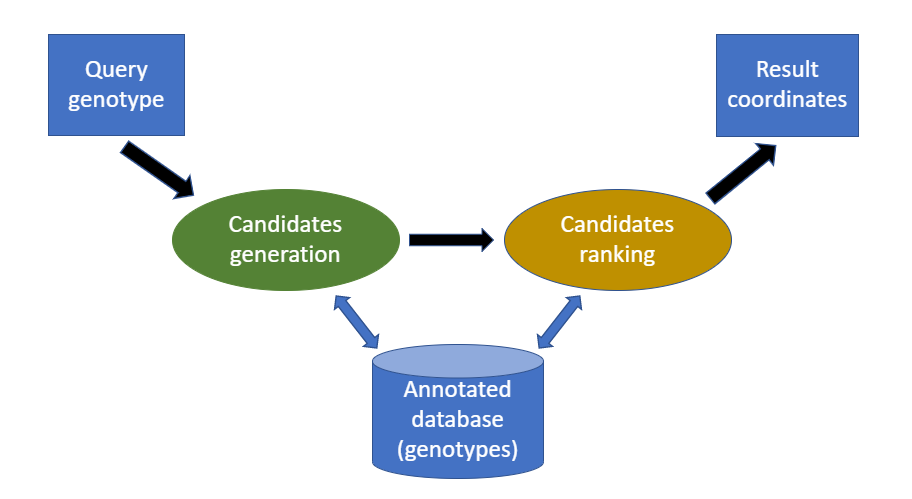
\includegraphics[width=14cm]{images/geoloc_over.png}
\end{center}
  \caption{Общая схема предложенных методов по геолокации.}
  \label{image:geoloc_over}
\end{figure}

В контексте модуля генерации координат-кандидатов можно рассмотреть два подхода. Первый подход
заключается в извлечении из тренировочной выборки координат всех известных генотипов,
их дедублицирования. Второй способ -- генерация узлов решетки, равномерно покрывающей
интересующую территорию (в данном случае территорию Республики Беларусь). Второй способ подразумевает
наличие параметра отвечающего за количество узлов решетки, что дает проектируемому методу
дополнительную степень свободы.

Рассмотрим следующие методы ранжирования координат-кандидатов:
\begin{itemize}
\item Случайный выбор $k$ кандидатов.

Нередко для анализа задач, а также установления пригодности метрик в различных задачах
используются базовые методы, поведение которых позволяет установить некоторые пороговые значения для метрик.
Для метрики ROC AUC в задаче бинарной классификации, например, также во внимание принимается
поведение случайного классификатора. Таким образом, хороший метод ранжирования должен давать лучшие значения по
метрикам в сравнении со случайным выбором.

\item Метод ближайшего соседа.

Среди генотипов тренировочной выборки, выполняется поиск наиболее близкого к генотипу запроса $g_{query}$:

$ j_{min} = arg\,min_{\left(g^j_{train}, c^j_{train}\right) \in X_{train}} ||g^j_{train} - g_{query}||$.

Полученный ближайший сосед из тренировочной выборки используется для ранжирования координат-кандидатов --
наибольший ранг присваивается координатам, наиболее близким $c^{j_{min}}_{train}$ к полученному ближайшему соседу.
В данном случае, в отличие от случайного выбора, принимается во внимание генотип-запрос. Также, используется довольно сильное
предположение о локальности генотипов (то есть в генотипах индивидов существует некоторая географически выраженная структура,
причем близость генотипов влечет их географическую близость). Один из примеров -- этногеографическая близость,
гипотеза о близости генотипов в пределах исторически сложившихся этнических регионов.

\item Упорядочивание в соответствии с генотипической близостью.

Каждому кандидату ставится в соответствие ближайший (географически) генотип из тренировочной выборки.
Кандидаты упорядочиваются на основе близости соответствующих их генотипов тренировочной выборки и генотипа-запроса $g_{query}$.
Основное отличие от метода ближайшего соседа - итоговые кандидаты могут быть распределены по интересующей нас территории, явное ограничение на локальность отсутствует.

\item Гибридное ранжирование кандидатов

Можно заметить, что все предыдущие методы задействовали только меру генотипической близости между кандидатами и тренировочной выборкой, а также
в целом влияние на ранг каждого кандидата оказывала лишь небольшая группа образцов тренировочной выборки.

Для некоторого генотипа-запроса $g_{query}$ и кандидата $c$ рассмотрим следующую функцию:

$$ F \left( g_{query}, c\right) = \langle G_{f} \left( G_{train}, g_{query}\right), D_{f} \left( C_{train}, c\right) \rangle $$

где $G_{f} \left( G_{train}, g_{query}\right)$ - оценивает генотипическую близость запроса и генотипов тренировочной выборки, $D_{f} \left( C_{train}, c\right)$ -
оценивает географическую близость образцов тренировочной выборки и координат кандидата. В качестве $G_{f}$ и $D_{f}$ предлагается брать нелинейные функции.
Предложенные реализацие функций $G_{f}$, $D_{f}$:

$$ G^0_{f} \left( G_{train}, g_{query}\right) = \sigma \left( \left( || G_{train} - g_{query} || - g_{mean} \right) g_{std} \right) $$
$$ G_{f} \left( G_{train}, g_{query}\right) =  \mathbbm{1} | G^0_{f} \left( G_{train}, g_{query}\right) > g_{threshold} | \cdot  G^0_{f} \left( G_{train}, g_{query}\right)$$
$$ D^0_{f} \left( C_{train}, c\right) =  \exp \left( - || C_{train} - c || * d_{alpha}\right)$$
$$ D_{f} \left( C_{train}, c\right) =  \mathbbm{1} | D^0_{f} \left( C_{train}, c\right) > d_{threshold} | \cdot  D^0_{f} \left( C_{train}, c\right) $$

Таким образом, функция $F$ дает нам возможность оценить некоторые генотип-запрос $g_{query}$ и кандидата $c$
используя всю тренировочную выборку, используя не только меры генотипической близости, но добавить к этому взвешивание
на основе географической близости.
\end{itemize}

\section{Практические результаты}

В качестве практических экспериментов была проведена оценка качества следующих комбинаций:
\begin{itemize}
\item Генератор: координаты генотипов из тренировочной выборки. Метод ранжирования: случайный выбор.

\item Генератор: координаты генотипов из тренировочной выборки. Метод ранжирования:
географическая близость к лучшему совпадению по генотипу.

\item Генератор: координаты генотипов из тренировочной выборки. Метод ранжирования: метод ближайших соседей.

\item Генератор: координаты генотипов из тренировочной выборки. Метод ранжирования: независимое ранжирование кандидатов.
Для нахождения оптимальных значений гиперпараметров $g_{mean}$, $g_{std}$, $g_{threshold}$, $d_{alpha}$, $d_{threshold}$
была использована байесовская оптимизация: для каждой отдельно взятой пары параметров $d$ и $k$, было выполнено 150 итераций (ввиду необходимости большого количества
вычислительных ресурсов). Также, основываясь на анализе предыдущих методов, для всех $k \ge 10$ было наложено явное ограничение на метрику покрытие $cov \ge 150$.
\end{itemize}

Сетка параметров $d$, $k$ состояла из следующих значений:
\begin{itemize}

\item $k$ - количество кандидатов. Значения: $[1, 3, 5, 10, 15, 20].$

\item $dt$ - выбранная погрешность. Значения: $[0.1, 0.3, 0.5, 1].$ Единица эквивалентна 111 км (радиальное расстояние).

\end{itemize}

Для перечисленных выше комбинаций была произведена оценка метрики hit probability
c использованием тренировочной выборки и кросс-валидации (20 фолдов). Результаты представлены на рисунке $\left(\ref{image:hit}\right)$.
Можно заметить, что метод упорядочивания в соответствии с генотипической близостью оказался лучше других предложенных методов. Также,
с ростом допустимой погрешности $d$, ввиду равномерного расположения кандидатов по территории, результаты случайного метода ранжирования становятся все лучше,
т.к. вероятность попадания в круг большего радиуса пропорциональна его размеру.
В данном случае это позволяет оценить перспективы использования предложенных методов на практике.
В целях тестирования и дальнейшего использования все описанные методы представлены в виде приложения с
 интерфейсом, который позволяет загрузить некоторый генотип (возможно частично)
и получить графическое представление результатов в виде тепловой карты (рисунок $\left(\ref{image:geoui}\right)$.).

\begin{figure}[h]
\begin{center}
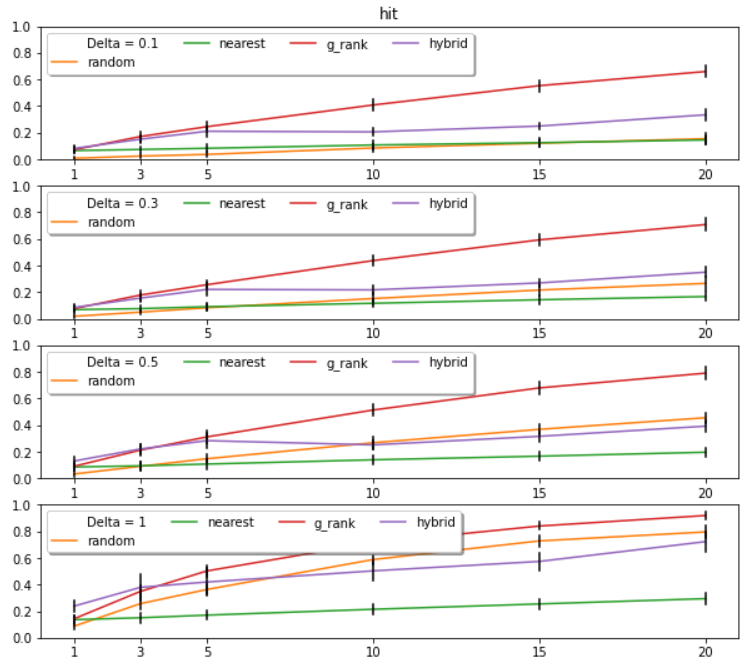
\includegraphics[width=14cm]{images/hit.png}
\end{center}
  \caption{Результаты тестирования методов геолокации на тренировочной выборке, метрика hit probability}
  \label{image:hit}
\end{figure}

\begin{figure}[h]
\begin{center}
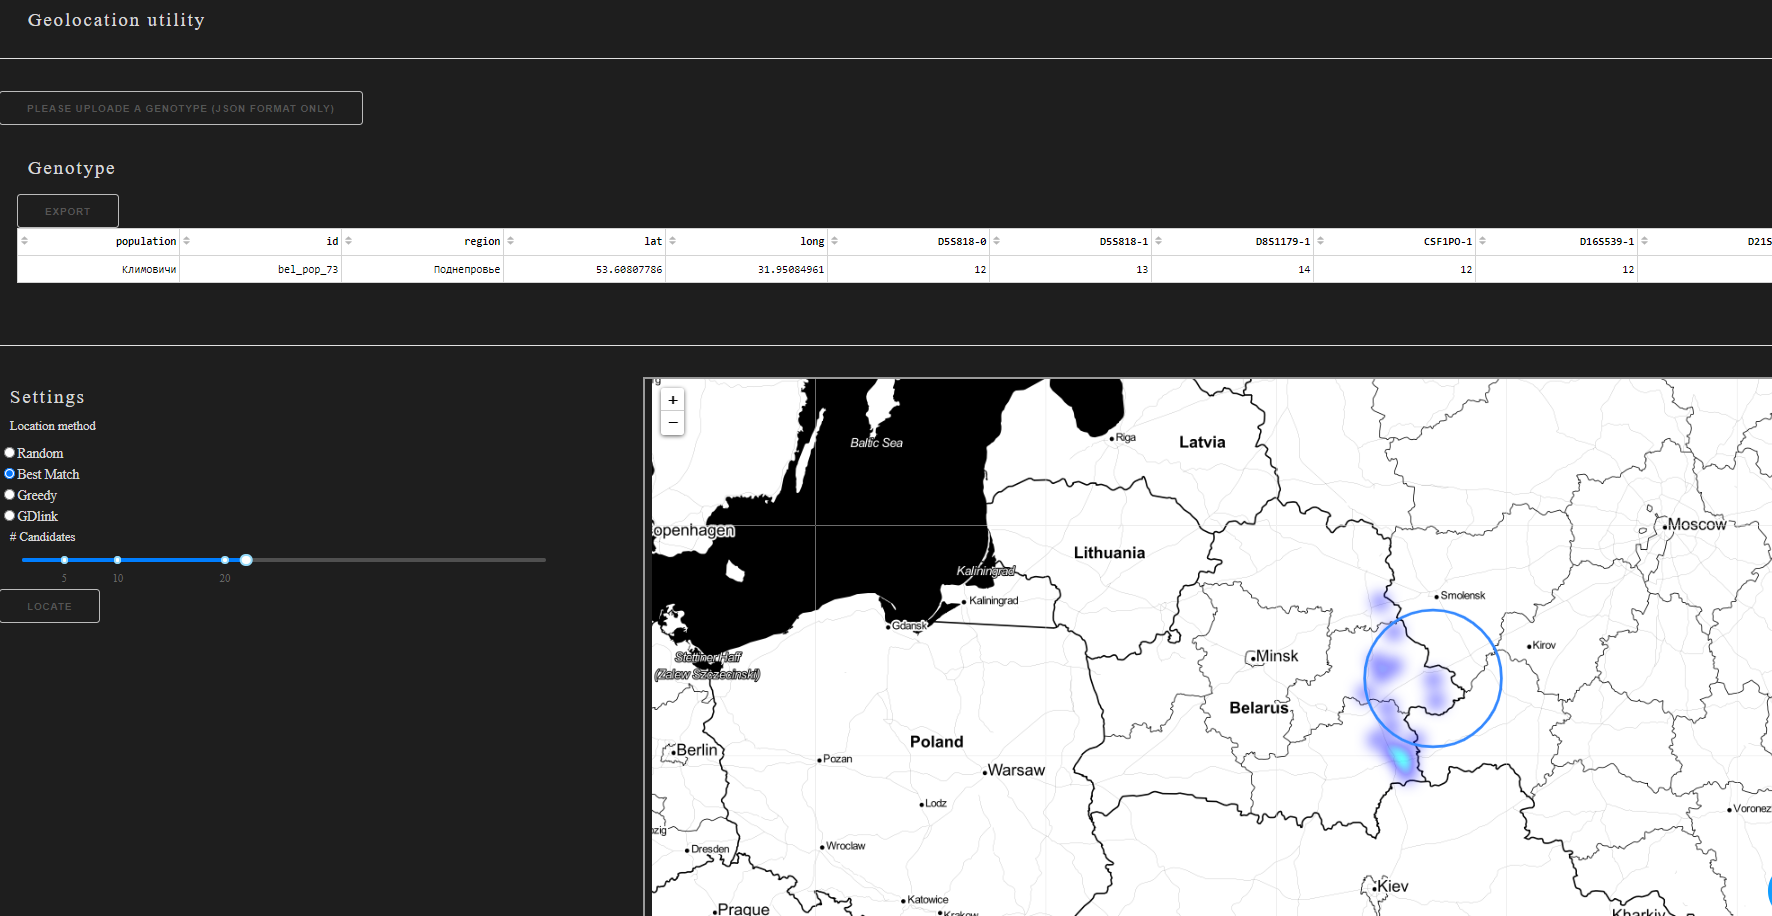
\includegraphics[width=14cm]{images/geoui.png}
\end{center}
  \caption{Приложение по геолокации генотипов}
  \label{image:geoui}
\end{figure}
